\section{Despliegue}

El despliegue del sistema fué realizado en dos procesos separados: El despliegue de la interfaz gráfica del sistema web, y el de el sistema de monitoreo y API. Esto se realizó debido a que las herramientas necesarias para el funcionamiento del API no eran accesibles desde la plataforma principal, por lo que se decidió dividir el proyecto y tenerlo en servidores independientes.

Para simplificar el proceso del sistema de despliegue de la interfaz gráfica, se creó un usuario en el servidor del sitio CECATEV para ahí depositar los archivos necesarios. Además, para utilizar la infraestructura existente de el Centro, se decidió crear una ruta dentro del sitio en la que fuera posible acceder al proyecto desarrollado. Para esto, se creó la carpeta \texttt{meteoreo} en la ruta \texttt{/var/www/html/}.

Después de crear la carpeta, se utilizó el gestor de paquetes para iniciar la compilación de un sitio para producción, con el comando \texttt{yarn build}, el cual fue configurado automáticamente gracias al framework. Este comando produce una versión del sitio web sin librerías extra y con mejoras de velocidad en comparación a su contraparte de desarrollo.

Por último, para enviar la versión de producción del sitio web al servidor, se utilizó la herramienta \textit{rsync}, la cuál fue seleccionada debido a su simpleza de uso, replicabilidad y compatiblidad con el protocolo SSH que es utilizado para acceder al servidor. Esta operación fué repetida múltiples veces durante el desarrollo del proyecto, y fué posible encapsularlo en una sóla línea de código, con la forma \texttt{yarn build \&\& rsync -avz dist/ -e ssh al142912@cecatev.uacj.mx:/var/www/html/meteoreo}. Un fragmento de este proceso puede ser observado en la Figura \ref{fig:uploading-web}.

\begin{figure}[!ht]
	\centering
	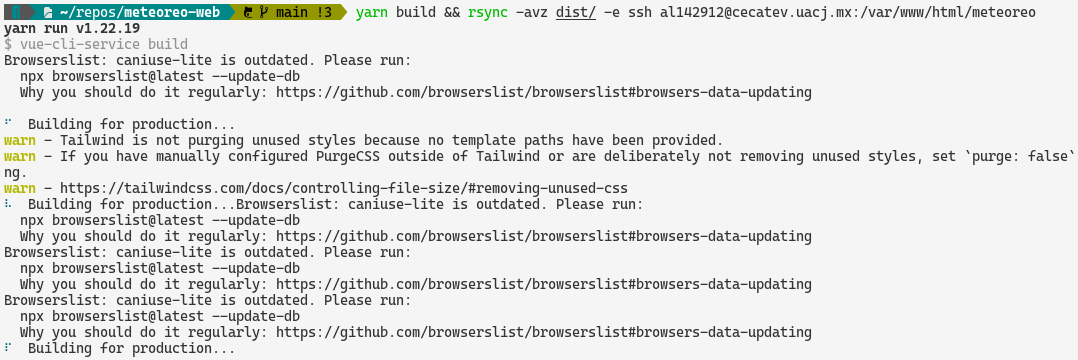
\includegraphics[width=0.9\linewidth]{images/screenshots/meteoreo-web-rsync-upload.png}
	\caption{Despliegue de la interfaz web.}
	\label{fig:uploading-web}
\end{figure}

El proceso de despliegue del API y servicio de monitoreo se realizó en un servidor diferente, una máquina virtual manejada por el instituto a la que se le asignaron 8GB de RAM, 8 núcleos del procesador Intel Xeon E5-4640 con una velocidad de 2.399GHz y 492GB de disco duro. En este servidor fué instalado el sistema operativo Ubuntu Server versión 18.04.6 LTS, y sobre este sistema operativo se configuró docker conforme a la guía oficial de Docker para la versión correspondiente del sistema. Cabe resaltar que por fines de asegurar una mejor conexión con las estaciones destinadas a ser monitoreadas, este servidor fue asignado al segmento de red perteneciente a estas, ocasionando que no fuera accesible desde la red pública, y para tener acceso se requiere del uso de una VPN.

Después de haberse instalado Docker, se instaló la utilería \textit{docker-compose}, para facilitar la configuración del sistema. Después que se configuraron estas herramientas, se descargó el código del repositorio con la herramienta Git en la carpeta \texttt{/opt/meteoreo-api}. Después de esto, se configuraron las variables de entorno correspondientes y se ejecutó el comando \texttt{docker-compose up} para arrancar el funcionamiento del servicio.

El servicio de monitoreo se decidió ejecutar en la misma imágen de Docker como un proceso manual, esto debido a que se podría facilitar el proceso de monitoreo y actualización. Por lo tanto, se dejó el proceso ejecutando en una ventana de \textit{tmux}, el cual permite crear terminales virtuales para ejecutar procesos sin afectar la terminal principal. Una nota importante es que el sistema se configuró para utilizar una instancia local de la base de datos MariaDB, esto debido a que el sistema que se desplegó será utilizado temporalmente para reivsar la estabilidad del mismo.

Como resultado de la configuración seleccionada es posible actualizar el sistema con una versión nueva con facilidad, como se puede observar en la Figura \ref{fig:uploading-web}, debido a que sólo es necesario actualizar el repositorio de Git para que los cambios se vean reflejados. Esto, a pesar de que es un proceso manual, agiliza el despliegue de nuevas versiones que solucionen problemas sin afectar el tiempo de respuesta al usuario final.

\begin{figure}[!ht]
	\centering
	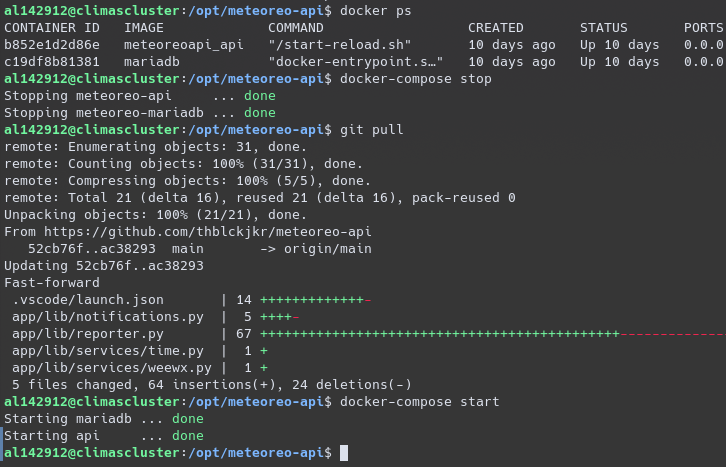
\includegraphics[width=0.9\linewidth]{images/screenshots/meteoreo-api-update.png}
	\caption{Actualización del API y servicio de monitoreo.}
	\label{fig:uploading-web}
\end{figure}

\section{Evaluación}

Para facilitar la evaluación de la calidad de la información del sistema, a este se le configuró el nivel de información en las variables de entorno con el nivel \texttt{INFO}, el cuál es el nivel mas informativo. Este nivel de información es útil para la verificación de un correcto funcionamiento del sistema, ya que contiene información detallada de los servicios monitoreados, respuestas de sistemas externos, así como información sobre la autenticación que se realiza, un ejemplo se de esta información se puede ver en la Figura \ref{fig:meteoreo-api-monitoring}.

\begin{figure}[!ht]
	\centering
	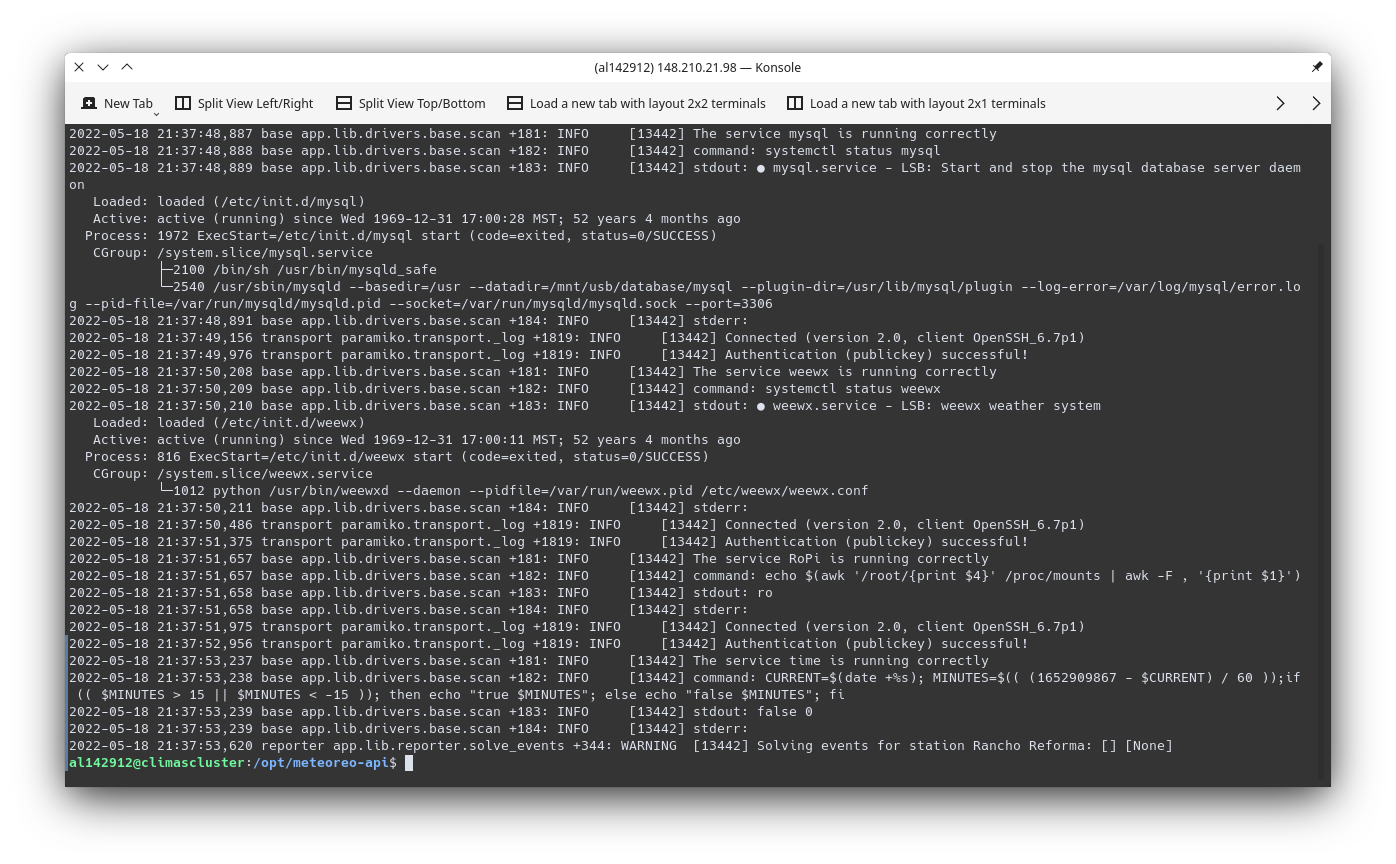
\includegraphics[width=1\linewidth]{images/screenshots/meteoreo-api-monitoring.png}
	\caption{Información de monitoreo.}
	\label{fig:meteoreo-api-monitoring}
\end{figure}

\section{Lanzamiento}

Este proyecto es de código libre, y fue publicado en Github bajo la licencia GPL-3.0. El API junto con el servicio de monitoreo puede encontrarse en el repositorio \href{https://github.com/thblckjkr/meteoreo-api}{thblckjkr/meteoreo-api} y el código de la interfaz web puede encontrarse en \href{https://github.com/thblckjkr/meteoreo-web}{thblckjkr/meteoreo-web}. Los hashes de commit específicos que se utilizaron para la muestra final bajo la que fué evaluada en este proyecto, es el \href{https://github.com/thblckjkr/meteoreo-api/tree/540ffcf1a00a6ad57887ec69a6095b5636a29806}{540ffc} para el repositorio meteoreo-api y el \href{https://github.com/thblckjkr/meteoreo-web/tree/08f56ba9712b3392244634dcbf0060c205d13f4f}{08f56ba} para meteoreo-web. Por último, la interfaz web es accesible desde el URL \href{http://cecatev.uacj.mx/meteoreo}{cecatev.uacj.mx/meteoreo}.
